\chapter{Supporting Materials}

% This would be any supporting material not central to the dissertation.
% For example:
% \begin{itemize}
% \item additional details of methodology and/or data;
% \item diagrams of specialized equipment developed.;
% \item copies of questionnaires and survey instruments.
% \end{itemize}

% \section{Symmetric Locomotion}


\section{\Cref{ch:envparams} Hyper-parameters}
\label{sec:envparam_hyperparams}

The following contains the hyper-parameters used for all of the experiments in \Cref{ch:envparams}. The code is also available under \url{https://github.com/farzadab/walking-benchmark/}.
\begin{table}[h]
    \centering
    \begin{tabular}{lc}
        \toprule
        Name & Description \\
        \midrule
        Policy LR & $3e^{-3}$\\
        Value Network LR & $5e^{-3}$\\
        Total Environment Steps & $6$ Million\\
        Clipping Parameter ($\epsilon$) & $0.2$\\
        Decay ($\gamma$) & $0.99$\\
        GAE $\lambda$ & $0.95$ \\
        Policy type & Fixed Diagonal Gaussian\\
        Policy stdev & $\exp(-1)$\\
        Network Size & 3 Layers of 256 nodes \\
        Network Activations & ReLU \\
        Max Grad Norm & 1\\
        Optimization Batch Size & $128$ \\
        PPO Optimization Steps & $10$ \\
        \bottomrule
    \end{tabular}
    \caption{Hyper-parameters used in \Cref{ch:envparams}.}
    \label{tab:envparam_hyperparams}
\end{table}

\section{Mirroring Functions}
\label{sec:mirroring-functions}

The mirroring functions, $\mathcal{M}_s$ and $\mathcal{M}_a$ as described in \Cref{sec:methods} are properties of the environment.  Consequently, the environment is responsible for providing the necessary information for policies to perform the mirroring operation on state and action.  Although the mirroring functions can be arbitrarily complex, we found that all the environments in \Cref{sec:environments} share a similar construction.  Using \textit{Walker3D} as an example, the method for deriving mirror functions are described in detail below.

The \textit{Walker3D} character has a total of 21-DoF and each DoF is modeled as a one-dimensional hinge joint.  Furthermore, let the \textit{x}-axis be the forward direction and the \textit{z}-axis pointing up in the local coordinate frame of the character.  For mirroring purposes, the joints can be divided into three categories, common, opposite, and side.  The common categories contain joints that are unchanged by the mirroring function, such as $abdomen_y$.  In general, joints that rotate about the \textit{y}-axis should remain unchanged after mirroring.  The opposite categories contains joints that are mainly on the torso of the character and they need to be negated for mirroring.  In the case of \textit{Walker3D}, only $abdomen_x$ and $abdomen_z$ would fall under this category.  The side categories contains joints that are on the limbs.  Importantly, for each joint on one side there must be a corresponding joint on the other side; for instance, the right knee corresponds to left knee.  With the one-to-one mapping, $\mathcal{M}_a$ can simply interchange the applied torques for the respective joints on either side.  We found that it is more straight-forward if the joint rotation axes are flipped, except for axes aligned on the  \textit{y}-axis, for the left and right limbs.  Otherwise, additional negation operation need to be applied after interchanging left and right actions. 

$\mathcal{M}_s$ follows a similar pattern as described above.  For state information that are derived from the character, such as joint angles and angular velocities, the mirrored counterpart would have negated and interchanged values.  In addition, the environment may provide additional information, such as character orientation, velocity, and target location in character root space, as in \textit{Walker3D}.  For vector-valued information, such as velocity and target location, the values along the $y$-axis should be negated; for orientations, values representing roll and yaw should be negated.

\section{Phase Plots}
\label{sec:phase-plots}

Phase plots, \Cref{fig:phase-plots}, for the \textit{Walker2D} and \textit{Walker3D} tasks are generated from the run that produced the most symmetric gait for each method.  

\begin{figure}
  \centering
  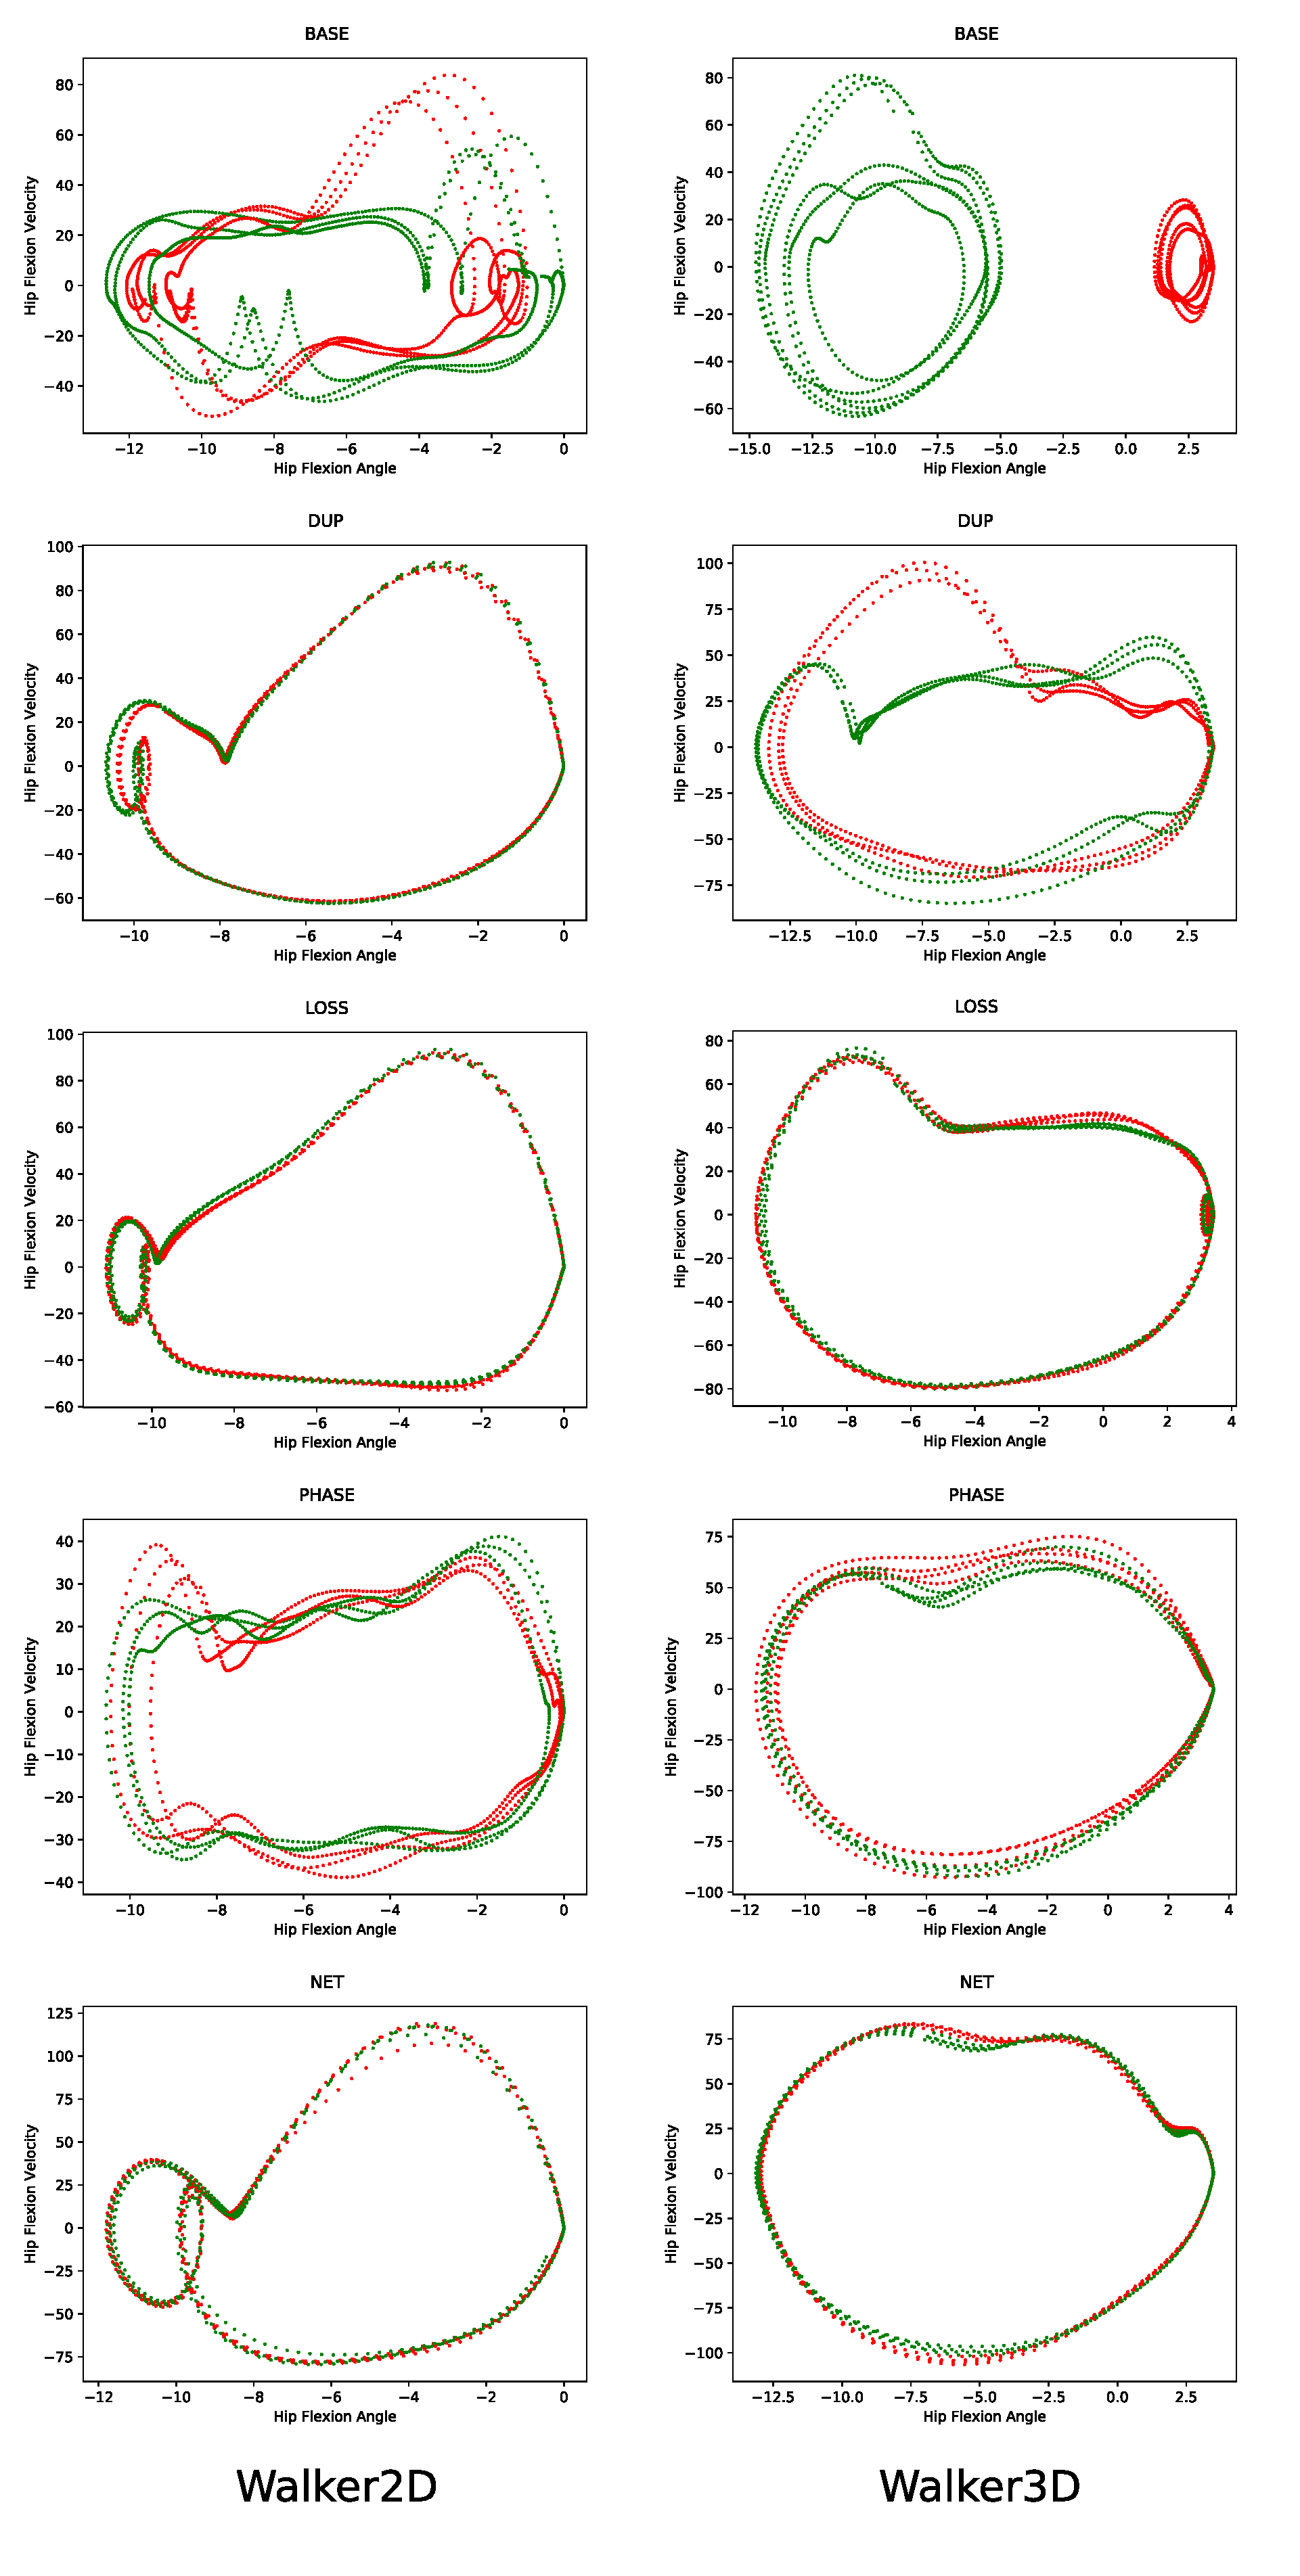
\includegraphics[width=0.70\columnwidth]{symmetry_figures/phase_plots.pdf}
  \caption{Phase Plots.  The green curve is for the left hip flexion, and red for the right side.  The more symmetric the motion, the more aligned are the curves.}
  \label{fig:phase-plots}
\end{figure}

\section{Alternate Symmetric Network Architecture}
\label{sec:alternate-network}

In \Cref{fig:net-architecture}, we presented a universal method for embedding any neural network into a symmetric policy.  The NET method effectively uses the same policy module twice with flipped inputs for $s$ and $M(s)$.  While this construction is relatively simple to implement, alternative symmetric policy constructions do exist.  In this section, we describe the construction used for NET-ALT in \Cref{fig:learning-curves}.



Recall that a symmetric policy is one that satisfies \Cref{eq:symmetric-policy}, along with the fact that our mirror functions (\Cref{sec:mirroring-functions}) essentially perform negation and swapping operation on the state and action vectors.  Let us then consider the individual layers of a neural network as matrix operations, in particular, before the application of non-linear activation functions.  The full matrix form of the first layer for $s$ and $\mathcal{M}_s(s)$ can be written as,

\begin{center}
$\begin{bmatrix} W \\ X \\ Y \\ Z  \end{bmatrix} = (a_{ij})_{4\times4} \begin{bmatrix} C \\ O \\ R \\ L \end{bmatrix}$ and, $\begin{bmatrix} W \\ -X \\ Z \\ Y  \end{bmatrix} = (a_{ij})_{4\times4} \begin{bmatrix} C \\  -O \\  L \\ R \end{bmatrix}$.
\end{center}

$C$, $O$, $R$, $L$ represent the portions of the state vector corresponding to common, opposite, right, and left respectively.  The uppercase letters for $C$, $O$, $R$, $L$, $W$, $X$, $Y$, and $Z$ indicate that these are not necessarily scalars. For instance, for \textit{Walker3D}, $O$ contains both $abdomen_x$ and $abdomen_z$.  Similarly, the matrix, $(a_{ij})_{4\times4}$, is dimensionally consistent with the corresponding elements in the state vector.  For example, $a_{2j}$ is a two-column wide block that matches with the two elements in $O$ for \textit{Walker3D}.  In addition, notice the negated $O$ and $X$, as well as the interchanged $R$ and $L$ are the effect of the mirroring functions.  Overall, there are a total of 16 unknowns and 8 equations.  A symmetric layer can be obtained by solving this system of equations.  In particular, \textit{NetAlt} contains symmetric layers of the following form,

\begin{center}
$(a_{ij})_{4\times4} = \begin{bmatrix} 
\alpha &  0 & \beta & \beta \\ 
0 & \gamma & \beta & -\beta \\
\delta &  \epsilon & \zeta & \eta \\
\delta & -\epsilon & \eta & \zeta
\end{bmatrix}$.
\end{center}

In order to maintain the symmetric policy constraint, the activation function applied to the negation portion, $O$, must be an odd function such as \textit{tanh} or \textit{softsign}.  A similar procedure can be followed for intermediate and output layers, as long as the sizes for each of the portions are correctly maintained.  Finally, a symmetric policy network can be constructed by stacking symmetric layers.

\section{Symmetry in DeepMimic Environment}
\label{sec:deepmimic-results}

To evaluate the effectiveness of phase-based mirroring, we ran an experiment for the original DeepMimic environment \citep{2018-TOG-deepMimic} in additional to the \textit{Cassie} environment.  In both cases, our data shows that phase-based mirroring does indeed make the learning faster.  However, in the case of \textit{DeepMimic}, the difference in final return is small between BASE and PHASE and only a minor difference can be gleamed from the video.

\begin{figure}
  \centering
  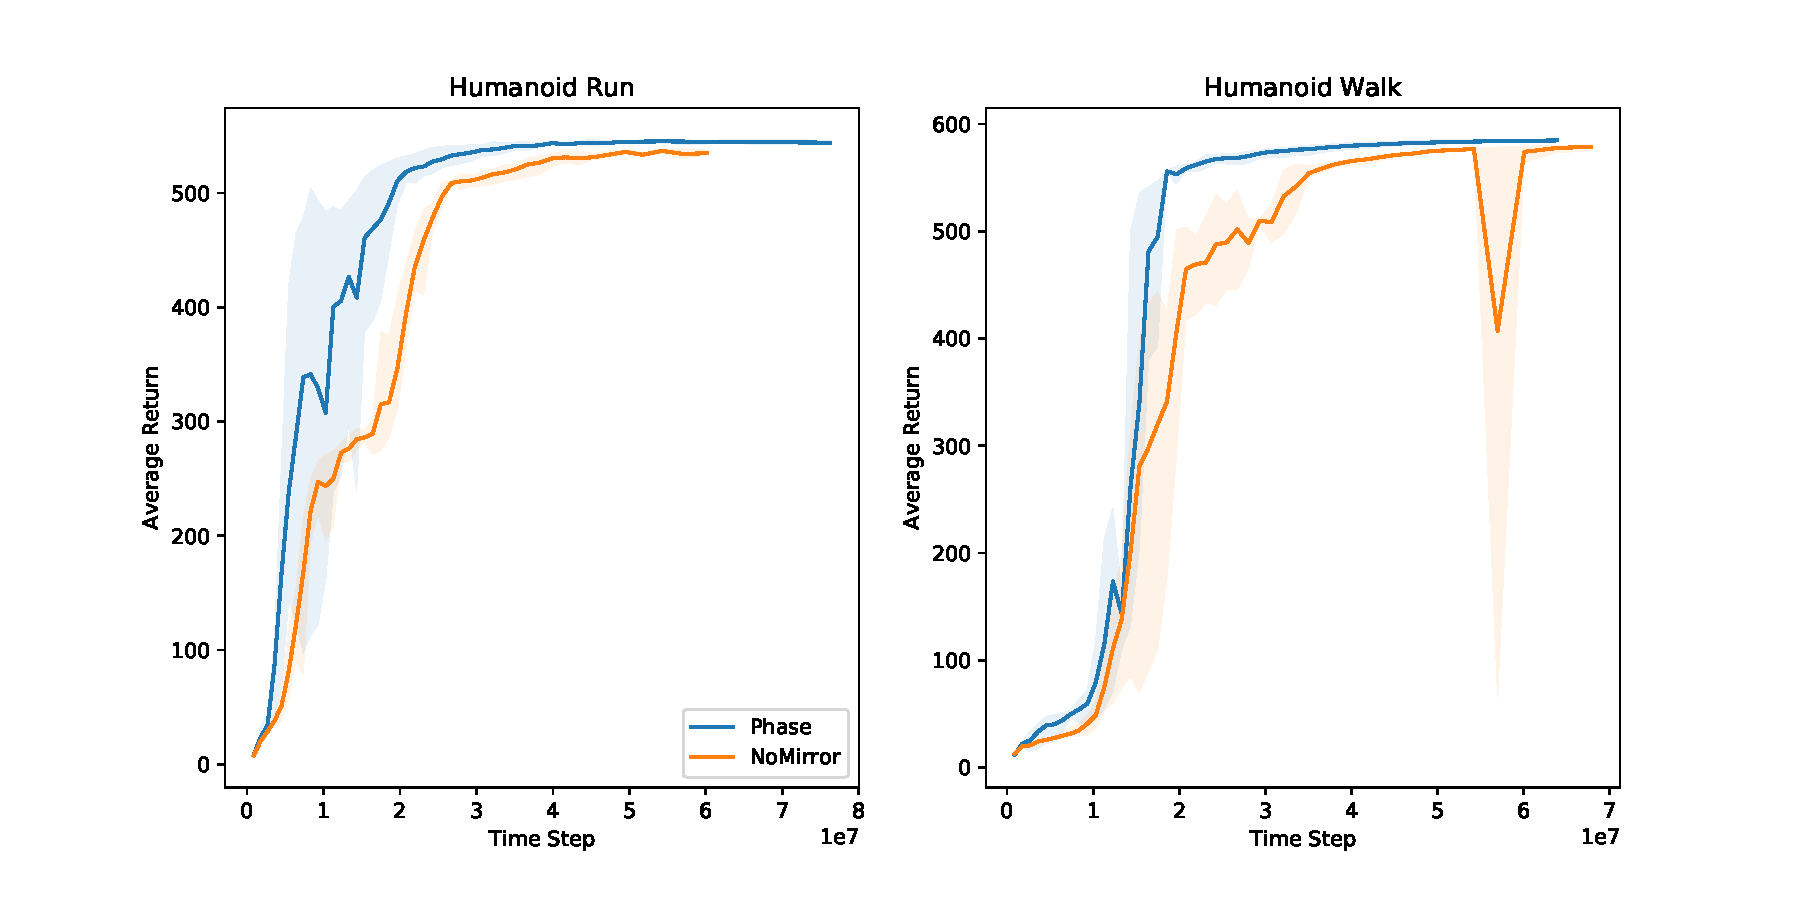
\includegraphics[width=0.9\columnwidth]{symmetry_figures/DeepMimic_curves.pdf}
  \caption{Learning curves for the original \textit{DeepMimic} environment. BASE and \textit{Phase} corresponds to the symmetry enforcement methods in \Cref{fig:learning-curves}.}
  \label{fig:deepmimic-curves}
\end{figure}